\documentclass[11pt]{article}

\usepackage[utf8]{inputenc} % allow utf-8 input
\usepackage[T1]{fontenc}    % use 8-bit T1 fonts
\usepackage{hyperref}       % hyperlinks
\usepackage{url}            % simple URL typesetting
\usepackage{booktabs}       % professional-quality tables
\usepackage{amsfonts}       % blackboard math symbols
\usepackage{nicefrac}       % compact symbols for 1/2, etc.
\usepackage{microtype}      % microtypography
\usepackage{booktabs}
\usepackage{caption}

\usepackage{booktabs} % For formal tables
\usepackage{tabulary}
\usepackage{makecell}
\usepackage{xfrac}
\usepackage[margin=0.75in]{geometry}
%\let\comment\relax
%\usepackage[authormarkup=none]{changes}

\usepackage{thm-restate}

\usepackage[ruled]{algorithm2e} % For algorithms
\renewcommand{\algorithmcfname}{ALGORITHM}
\newcommand\mycommfont[1]{\footnotesize\ttfamily\textcolor{blue}{#1}}
\SetCommentSty{mycommfont}

\SetKwInput{KwInput}{Input}                % Set the Input
\SetKwInput{KwOutput}{Output}  

\SetAlFnt{\small}
\SetAlCapFnt{\small}
\SetAlCapNameFnt{\small}
\SetAlCapHSkip{0pt}
\SetKwInput{KwEl}{Elicitation Rule}
\SetKwInput{KwAgg}{Aggregation Rule}
\SetKwInput{KwComm}{Communication Complexity}
\SetKwInput{KwDist}{Distortion}
\IncMargin{-\parindent}

\usepackage{color}
\usepackage{amsmath,amsthm,amsfonts,amssymb,bbm}
\usepackage{enumitem}
\usepackage[english]{babel}
\usepackage{multirow}
\renewcommand*\ttdefault{cmtt}

\newtheorem{definition}{Definition}
\newtheorem{theorem}{Theorem}
\newtheorem{conjecture}{Conjecture}
\newtheorem{lemma}{Lemma}
\newtheorem{proposition}[theorem]{Proposition}
\newtheorem{corollary}[theorem]{Corollary}

\usepackage{graphicx}
\usepackage{cleveref}


% COMMENTS
\newcount\Comments  % 0 suppresses notes to selves in text
\Comments = 1
\newcommand{\kibitz}[2]{\ifnum\Comments=1{\color{#1}{#2}}\fi}
\newcommand{\dm}[1]{\kibitz{magenta}{[Deb: #1]}}
\newcommand{\sd}[1]{\kibitz{blue}{[Sam: #1]}}

%\renewcommand{\citet}[1]{\citeauthor{#1}~\cite{#1}}

% MATH - GENERIC
\newcommand{\ceil}[1]{\lceil #1 \rceil}
\newcommand{\floor}[1]{\lfloor #1 \rfloor}
\newcommand{\sign}{\textrm{sign}}
\newcommand{\supp}{\textrm{supp}}
\renewcommand{\hat}{\widehat}
\newcommand{\E}{\mathbb{E}}
\renewcommand{\tilde}{\widetilde}
%\renewcommand{\vec}{\mathbf}
\newcommand{\set}[1]{\{#1\}}

\newcommand{\calC}{\mathcal{C}}
\newcommand{\calE}{\mathcal{E}}
\newcommand{\calH}{\mathcal{H}}
\newcommand{\calL}{\mathcal{L}}
\newcommand{\calP}{\mathcal{P}}
\newcommand{\calQ}{\mathcal{Q}}
\newcommand{\calS}{\mathcal{S}}
\newcommand{\calX}{\mathcal{X}}
\newcommand{\calY}{\mathcal{Y}}

\newcommand{\bbR}{\mathbb{R}}
\newcommand{\bbN}{\mathbb{N}}

\DeclareMathOperator*{\argmin}{arg\,min}
\DeclareMathOperator*{\argmax}{arg\,max}

% CS - COMPLEXITY
\newcommand{\bigo}[1]{O\left(#1\right)}%
\newcommand{\bigom}[1]{\Omega\left(#1\right)}%
\newcommand{\bigolog}[1]{\tilde{O}\left(#1\right)}%

% PAPER SPECIFIC
\newcommand{\query}{\calQ}
\newcommand{\complist}{\calP}
\newcommand{\comp}{P}
\newcommand{\eli}{\Pi}
\newcommand{\agg}{\Gamma}
\newcommand{\comm}{\textrm{C}}
\newcommand{\dist}{\textrm{dist}}
\renewcommand{\sc}{\textrm{sc}}
\newcommand{\nsw}{\textrm{nsw}}
\newcommand{\sw}{\textrm{sw}}
\newcommand{\hsw}{\hat{\sw}}
\newcommand{\hvi}{\hat{v}_i}
\newcommand{\id}{\mathbbm{1}}
\newcommand{\vv}{\vec{v}}
\newcommand{\vrho}{\vec{\rho}}
\newcommand{\vsigma}{\vec{\sigma}}

\newcommand{\ov}{\vv}
\newcommand{\vis}{\tilde{v}_i(S)}


\newcommand{\hata}{\hat{a}}
\newcommand{\WW}{\mathcal{W}}


\newcommand{\nhi}{N_{\text{high}}}
\newcommand{\nlo}{N_{\text{low}}}
\newcommand{\ahat}{\hat{a}}
\newcommand{\astar}{a^*}
\newcommand{\atilde}{\tilde{a}}
\newcommand{\qstar}{q^*}
\newcommand{\bx}{\mathbf{x}}
\newcommand{\abs}[1]{\left|#1\right|}
\newcommand{\UX}{\mathcal{X}}
\newcommand{\GFDISJ}{\mathrm{GFDISJ}}
\newcommand{\FDISJ}{\mathrm{FDISJ}}
\newcommand{\DISJ}{\mathrm{DISJ}}
\newcommand{\ent}{\mathrm{H}}
\newcommand{\mi}{\mathrm{I}}
\newcommand{\KL}{\mathrm{D_{KL}}}
\newcommand{\ic}{\mathrm{IC}}
\newcommand{\bstp}{\bar{s}_t'}
\newcommand{\ou}{\vec{u}}
\newcommand{\os}{\vec{\sigma}}
\newcommand{\low}{\textrm{low}}
\newcommand{\high}{\textrm{high}}
\newcommand{\RD}{R_{\delta}}

\newcommand{\Xc}{\mathcal{X}}
\newcommand{\Ac}{\mathcal{A}}
\newcommand{\Yc}{\mathcal{Y}}
\newcommand{\dd}{\mathcal{D}}
\newcommand{\reg}{\mathrm{Reg}}
\newcommand{\poi}{\mathrm{Poi}}
\newcommand{\eye}{\mathbf{1}}
\newcommand{\HH}{\mathcal{H}}
\newcommand{\YY}{\mathcal{Y}}

\newcommand{\eps}{\varepsilon}

\newcommand{\norm}[1]{\lVert #1 \rVert}
\hypersetup{
	colorlinks,
	linkcolor=red,
	citecolor=blue,
	urlcolor=green
}

\renewcommand\theequation{{\color{red}\arabic{equation}}}
%bib
\usepackage[style=alphabetic,natbib=true,backend=bibtex,backref=true,maxbibnames=10]{biblatex}
\addbibresource{./newrefs.bib}
\renewcommand{\cite}{\parencite}

\title{{\bfseries Fairness Checking} }
\begin{document}

\maketitle


\section{Introduction}
Nowadays, AI systems are increasingly used in various high-stakes decision making scenarios. Applications include bail decision, credit approval, and housing allocation, to name a few. These applications use learning algorithms trained on past data. However, past data is almost always biased in some way, and such bias is often reflected in the eventual decision. For example, \citet{BCZS+16} show that popular word embeddings implicitly encode societal biases, such as gender norms. Similarly, \citet{BG18} evaluate existing facial recognition systems and find that they perform better on lighter-skinned subjects as a whole than on darker-skinned subjects as a whole with an 11.8\% - 19.2\% difference in error rates. To mitigate these biases, there have been several approaches in the ML fairness community to design fair classifiers \cite{ZWSP+13,HPS16,ABDL+18}. Nonetheless, since different algorithms adopt different definitions of fairness and provide different trade-offs with respect to accuracy and utility, it is neither legal nor ethical to enforce businesses to use such algorithms. In this paper, we approach this problem with a perspective from the literature of automated verification, and aim to build tools that can verify whether an algorithm satisfies a given fairness criteria irrespective of the particular algorithm or dataset used. We show using these tools that, although current group fairness algorithms may mitigate fairness for a specific distribution of data, slight perturbations to that data's distribution result in violations of the fairness criteria. 

\section{Model}
We first check whether an algorithm is fair against a family of possible distributions. In particular, we consider distributions which are weighted empirical distributions and weights are chosen so that the new weighted distribution is close to the original training distribution.

\subsection{Setup}
Suppose, we have access to a ``protected'' attribute $A \in \set{0,1}$, and a qualification attribute $Y \in \set{0,1}$. In practice, a ``protected'' attribute might be race, gender, or some other attribute that might yield biased decision-making. Let us assume that $X \in \Xc$ denotes the set of remaining attributes which are used as input to a classifier $f$. For a distribution $P$ over the space of attributes $\Xc$, we consider the following two fairness criteria:
\begin{itemize}
\item Demographic Parity ({\bfseries DP}):
$$\abs{\E_{P}[f(X,a)|A=a] - \E_P[f(X,a')|A=a']} \le \epsilon$$
for all $a$ and $a'$.
\item Equalized Odds ({\bfseries EO}):
$$\abs{\E_{P}[f(X,a)|Y=y, A=a] - \E_P[f(X,a')|Y=y, A=a']} \le \epsilon$$
for all $y,a,$ and $a'$.
\end{itemize}
We assume that we have data $(X_i,Y_i,A_i)$ for $i=1,\ldots,n$ and $P$
can be represented as a weighted empirical distribution i.e. for any $(x,y,a) \in \Xc \times \set{0,1} \times \set{0,1}$ we have:
$$ P(x,y,a) = \sum_{i=1}^n w_i \eye_{(X_i,Y_i,A_i)=(x,y,a)}.$$
where the weights are specified with a weight vector $w = (w_1, ..., w_n)$ such that $w_i \geq 0$ for all $i$ and $\sum_i w_i = 1.$ 

\par

The two fairness definitions above are fairly standard and well-known in the fair ML literature. Both are examples of "group fairness." Demographic Parity, also known as Statistical Parity or Independence, \cite{DBLP:journals/corr/abs-1104-3913} means that the difference in positive rates for the two groups ("protected" and "unprotected") differ by some small $\epsilon.$ Equalized Odds, also called Positive Rate Parity or Separation, requires the two groups' true positive and false positive rates differ by some small $\epsilon.$

\subsection{Checking Demographic Parity (DP)}
As a start, we assume that the weighted empirical distributions are such that the marginal distributions over the protected attributes are preserved. In particular, we consider weights such that $\sum_{i=1}^n w_i \eye_{A_i = a} = \pi_a$ for all $a$. Here the $\pi_a$ are the proportions for the protected attributes, which we assume are known. We use the following linear programs to check if the classifier $f$ fails the fairness criterion on some allowable weighted empirical distribution. For each $a, a'$:
\begin{equation}
\label{eq:checkdp}
\begin{aligned}
\max_w \quad & \frac{1}{\pi_a} \sum_{i=1}^n w_i f(X_i)\eye_{A_i = a} - \frac{1}{\pi_{a'}} \sum_{i=1}^n w_i f(X_i)\eye_{A_i = a'} \\
\textrm{s.t.} \quad & \sum_{i=1}^n w_i \eye_{A_i = a} = \pi_a \\
& \sum_{i=1}^n w_i \eye_{A_i = a'} = \pi_{a'} \\
& w_i \ge 0 \quad \forall i \in [n] \\
&\sum_{i=1}^n w_i = 1
\end{aligned}
\end{equation}
If there exists a pair of protected attributes $a,a'$ such that the optimal value of the linear program is more than $\epsilon$, then we have found a violation of DP.

\subsection{Checking Equalized Odds (EO)}
As in the previous section, we assume that we only care about weighted empirical distributions such that $\sum_{i=1}^n w_i \eye_{A_i = a, Y_i = y} = \pi_{a,y}$ for all $a$ and $y$ where $\pi_{a,y}$ are known proportions for the protected and qualification attributes. We again use the following linear programs to check if $f$ fails the fairness criterion on some weighted empirical distribution.
\begin{equation}
\label{eq:checkeo}
\begin{aligned}
\max_w \quad & \frac{1}{\pi_{a,y}} \sum_{i=1}^n w_i f(X_i)\eye_{A_i = a, Y_i = y} - \frac{1}{\pi_{a',y}} \sum_{i=1}^n w_i f(X_i)\eye_{A_i = a',Y_i = y} \\
\textrm{s.t.} \quad & \sum_{i=1}^n w_i \eye_{A_i = a, Y_i = y} = \pi_{a,y} \\
& \sum_{i=1}^n w_i \eye_{A_i = a', Y_i = y} = \pi_{a',y} \\
& w_i \ge 0 \quad \forall i \in [n] \\
&\sum_{i=1}^n w_i = 1
\end{aligned}
\end{equation}
Like in DP, if there exists a pair of protected attributes $a,a'$ such that the optimal value of the linear program is more than $\epsilon$, then we have found a violation of DP.

\section{Evaluation}
Using the above framework, we evaluated the two group fairness properties (DP and EO) on two real world datasets used frequently in the fairness literature: Adult \cite{Adult} and COMPAS \cite{COMPAS}. We evaluated the robustness of classifiers satisfying DP and/or EO to perturbations in the original training distributions, given by some weighted empirical distribution. First, we trained fair classifiers on each of the datasets using well-known preprocessing techniques to achieve Demographic Parity and Equalized Odds within an acceptable $\epsilon$. Then, we allowed the weights of the empirical distribution to vary within a small margin of $\epsilon.$ Taking the first empirical weighting such that $\epsilon \geq 0.10,$ we analyzed the new marginal distributions of the data and compared it with the original marginal distribution of the data. 
%Let's avoid the term fair distribution
We found that very small changes in the marginal distributions of the data led to the classifier violating $\epsilon,$ suggesting the existing fair classifiers are not robust. 

\subsection{Datasets}
In our experiments, we use two real-world datasets: Adult and COMPAS. The Adult dataset consists of 14 attributes (e.g. age, education level, etc.) and 48,842 instances, used for predicting whether income exceeds \$50K/year based on U.S. Census data. The binary label ($Y$) in this dataset is positive if the subject's income exceeds \$50K/year USD and is negative if the subject's income is less than \$50K/year USD. For this dataset, we consider sex as the binary protected attribute ($A$), which is either Male ($A = 1$) or Female ($A = 0$). The COMPAS dataset consists of 53 attributes (e.g. race, age, prior offenses) and 7,214 instances, used for predicting whether a criminal defendant will recidivate. The binary label in this dataset is positive if the subject recidivated after two years and negative if they did not recidivate. For COMPAS, we consider race as the binary protected attribute, which is either Caucasian or not Caucasian. 
\par
For the rest of this paper, we refer to the sex in the Adult dataset and race in the COMPAS dataset as the protected attribute, denoted by $A.$ For the Adult dataset, we refer to Male as privileged class and Female as the non-privileged class, taking on values $A = 1$ and $A = 0,$ respectively. For the COMPAS dataset, we refer to Caucasian as the privileged class and not Caucasian (e.g. African-American, Hispanic, etc.) as the non-privileged class, taking on values $A = 1$ and $A = 0,$ respectively.

\subsection{Experimental Setup}
%\dm{Clarify what preprocessing does.}%
First, after doing standard preprocessing on the data (removing missing rows, feature selection, etc.) down to 45,222 instances for Adult and 6,172 instances for COMPAS,  we trained logistic regression (LR) classifiers on each by using the Optimized Pre-processing algorithm proposed by \citet{CWVN+17}. Optimized Pre-processing uses a probabilistic framework that determines an optimal random mapping of the training dataset into a transformed dataset used to train the model. This method is model agnostic because it is a preprocessing technique and is shown by Calmon et. al. to perform competitively well compared to other fair preprocessing algorithms in the literature with respect to group fairness. In our implementation, this preprocessing algorithm achieves Demographic Parity and Equalized Odds as desired on both datasets, while maintaining a reasonable classification accuracy. We use  $\delta_{DP}$ and $\delta_{EO}$ to denote the unfairness gap for DP and EO respectively.
\begin{align}
    \abs{\E_{P}[f(X,a)|A=a] - \E_P[f(X,a')|A=a']} := \delta_{DP} \\
    \abs{\E_{P}[f(X,a)|Y=1, A=a] - \E_P[f(X,a')|Y=1, A=a']} := \delta_{EOY1} \\
    \abs{\E_{P}[f(X,a)|Y=0, A=a] - \E_P[f(X,a')|Y=0, A=a']} := \delta_{EOY0}
\end{align}
For COMPAS, standard logistic regression classifier achieved $\delta_{DP} = 0.17, \delta_{EOY0} = 0.12,$ and $\delta_{EOY1} = 0.12$ with an accuracy of 0.66; whereas the optimized pre-processing algorithm proposed by \cite{CWVN+17} achieved $\delta_{DP} = 0.02, \delta_{EOY0} = 0.09,$ and $\delta_{EOY1} = 0.05$ with an accuracy of 0.64. For Adult, standard  logistic regression classifier achieved $\delta_{DP} = 0.21, \delta_{EOY0} = 0.11,$ and $\delta_{EOY1} = 0.46$ with an accuracy of 0.81; and the Optimized Pre-processing achieved $\delta_{DP} = 0.06, \delta_{EOY0} = 0.01,$ and $\delta_{EOY1} = 0.03$ with an accuracy of 0.79. Because, the  Optimized Pre-processing achieved an "unfairness gap" of under 0.1 with a minimal reduction in accuracy, we use this classifier as the base fair classifier for our experiments. %\dm{right?}%
%carried on our experiment using the LR classifier after Optimized Pre-processing on these datasets.  

\par
%\dm{I thought we first run the optimized preprocessing algorithm, and then use the LP on the resulting classifier. Probably you meant running Cal+17..}%
After running the Optimized Pre-processing algorithm to train a fair logistic regression classifier on Adult and COMPAS with respect to Demographic Parity and Equalized Odds, we make use of our linear programs in Section 2.2 and Section 2.3. For both Demographic Parity and Equalized Odds, we follow the constraints in (1) and (2), but we add one more constraint:
\begin{align}\label{eq:gamma-constraint}
    \frac{1 - \gamma}{n} \leq w_i \leq \frac{1 + \gamma}{n}
\end{align}
where $\gamma \in (0,1)$ is a parameter we use to set how much or how little $w_i$ can vary in our linear program. Note that, at $\gamma = 0,$ we simply have $w_i = \frac{1}{n},$ the original empirical distribution on the data. The parameter $\gamma$ allows us to control the distance between the weighted empirical distribution and the original distribution. Note that if the constraint \cref{eq:gamma-constraint} is satisified by all the training instances, the L1 norm between the weighted empirical distribution and the original distribution is at most $\gamma$. 
%By loosening this constraint, our linear program allows us to check weighted empirical distributions where our objective value (and, thus, our fairness property) takes violating values. 
\par
\textbf{Demographic Parity:} We aim to find the a value of $\gamma$ where our weighted empirical distribution first violates Demographic Parity with $\epsilon > 0.1.$ That is, by loosening the $\gamma$ in the bound in (6) on $w_i,$ we aim to find the first $\gamma$ such that our objective function violates:
\begin{align}
    \max_w \quad & \frac{1}{\pi_a} \sum_{i=1}^n w_i f(X_i)\eye_{A_i = a} - \frac{1}{\pi_{a'}} \sum_{i=1}^n w_i f(X_i)\eye_{A_i = a'} > 0.1 = \epsilon
\end{align}
subject to all the constraints before. Particularly, we test $\gamma \in \{0, 0.01, 0.02, ..., 0.98, 0.99, 1.0\}.$ Then, on the distribution of $w_i$ where $\epsilon > 0.1$ for our objective function, we analyze the marginal distributions on the attributes of our new, "unfair" empirical distribution. 
We measure the differences between the marginal distributions of the original distribution and the weighted unfair distributions to get an idea how different the distributions are, and how robust the fair classifiers are to perturbations in the training distribution.
%By comparing these marginal distributions to the original "fair" empirical distribution where $\gamma = 0$ and $w_i = \frac{1}{n},$ we aim to find the difference in the distributions needed for (7) to violate Demographic Parity fairness. 
These results are detailed in Section 3.3.
\par
\textbf{Equalized Odds:} We also aim to find a value of $\gamma$ where our weighted empirical distribution first violates Equalized Odds with $\epsilon > 0.1.$ In the context of Equalized Odds, this means the following:
\begin{align}
    \max_w \quad & \frac{1}{\pi_{a,0}} \sum_{i=1}^n w_i f(X_i)\eye_{A_i = a, Y_i = 0} - \frac{1}{\pi_{a',0}} \sum_{i=1}^n w_i f(X_i)\eye_{A_i = a',Y_i = 0} > 0.1 = \epsilon \\ 
    \max_w \quad & \frac{1}{\pi_{a,1}} \sum_{i=1}^n w_i f(X_i)\eye_{A_i = a, Y_i = 1} - \frac{1}{\pi_{a',1}} \sum_{i=1}^n w_i f(X_i)\eye_{A_i = a',Y_i = 1} > 0.1 = \epsilon
\end{align}
where (8) represents the difference in false positive rates ($Y = 0, f(X) = 1$) and (9) represents the difference in true positive rates ($Y = 1, f(X) = 1$), and the constraints for Equalized Odds are as before. Like in Demographic Parity, we test $\gamma$ in the range $\{0, 0.01, 0.02, ..., 0.98, 0.99, 1.0\}$ and find a distribution of $w_i$ where $\epsilon > 0.1.$ We compare this new, "unfair" empirical distribution through its marginal distributions to the original, "fair" empirical distribution. These results are detailed in Section 3.3.

\subsection{Results}
%Finally, to interpret the experiment's results, we analyzed each marginal distribution on the "unfair" reweighted attributes and compared them to the original marginal distributions from the "fair" distribution. To do this, we used L1-distance $D$ for each attribute. 
We measure the $L1$-distance between the marginal distributions over the attributes for the original distribution and the weighted ``unfair'' weighted distribution.
Because each feature was binary, the L1 distance for attribute $x$ was simply given by:
\begin{align}
    D_x = \abs{\Pr_w[x = 1] - \Pr_o[x = 1]} + \abs{\Pr_w[x = 0] - \Pr_o[x = 0]}
\end{align}
where $\Pr_w[x = n]$ is the marginal distribution from the reweighted, violating distribution and $\Pr_o[x = n]$ is the marginal distribution from the original, fair distribution. In Table 1 and Table 2 below, we summarize the results for a selected subset of attributes for each experiment. 

\begin{table}[htbp]
\small
\captionsetup{font=small}
\begin{tabular}{lllllllllllll}
\hline
COMPAS & $\gamma$ & sex    & age\_25 & age\_25\_45 & age\_45 & priors\_0 & priors\_1\_3 & priors\_3 & Avg. Dist.\\ \hline
DP        & 0.14 & 0.0014 & 0.0018  & 0.0042      & 0.0060  & 0.0010    & 0.015        & 0.025    & 0.0090 \\ \hline
EO, Y = 0 & 0.32 & 0.0040 & 0.016   & 0.0089      & 0.025   & 0.0065    & 0.020        & 0.014    & 0.015     \\ \hline
EO, Y = 1 & 0.19 & 0.0062 & 0.0053  & 0.0014      & 0.0038  & 0.013     & 0.0067       & 0.020    & 0.0071    \\ \hline
\end{tabular}
\caption{L1 distance from fair to "unfair" marginal distributions for COMPAS. $\gamma$ is the smallest value of $\gamma$ in constraint (6) to make LP difference (unfairness) $\geq$ 0.1. Selected attributes on display: \texttt{sex} is the sex of the individual, \texttt{age\_n} attributes are age < 25, 25 < age < 45, and age > 45, \texttt{priors\_n} means prior crimes = 0, 1 < prior crimes < 3, and 3 < prior crimes. Avg. Dist. is the average L1 distance through \textit{all} the features (some not shown here). } 
\label{tab:compas_results}

\medskip 

\begin{tabular}{lllllllllll}
\hline
Adult      & $\gamma$ & race   & age\_20 & age\_40 & age\_60 & edu6    & edu8    & edu10 & edu12 & Avg. Dist.  \\ \hline
SP         & 0.49  & 0.0049 & 0.021   & 0.017   & 0.0012  & 0.0055  & 0.0015  & 0.031 & 0.0052 & 0.014 \\ \hline
EO (Y = 0) & 0.47  & 0.0019 & 0.0060  & 0.00051 & 0.00064 & 0.0027  & 0.00064 & 0.011 & 0.00039 & 0.0033 \\ \hline
EO (Y = 1) & 0.17  & 0.0021 & 0.0021  & 0.0026  & 0.00042 & 0.00079 & 0.00051 & 0.012 & 0.00135 & 0.0036 \\ \hline
\end{tabular}
\caption{L1 distance from fair to "unfair" marginal distributions for Adult. $\gamma$ is the smallest value of $\gamma$ in constraint (6) to make LP difference (unfairness) $\geq$ 0.1. Selected attributes on display: \texttt{race} is the race of the individual (binary, White or not White), \texttt{age\_n} attributes are 20 < age < 30, 40 < age < 50, and 60 < age < 70, \texttt{edu\_n} means years of education total. Avg. Dist. is the average L1 distance through \textit{all} the features (some not shown here).}
\label{tab:my-table}
\end{table}

We observe that, by modifying the original "fair" distribution with uniform weights to a weighted empirical distribution that violates fairness for both properties (with gap $\ge 0.1$), the distributions are, in fact, extremely similar. The average L1 distance in marginal distributions between features in the original distribution and the violating distribution are all within the range of 0 and 1.5\%. For COMPAS DP, the maximum L1 difference in marginal distributions was 2.5\% for $\texttt{priors\_3}$ and for COMPAS EO, the maximum L1 differences were 2.5\% ($\texttt{age\_45}$, $Y = 0$) and 2.0\% ($\texttt{priors\_3}$, $Y = 1$). For Adult DP, the maximum L1 difference in marginal distributions was 8.8\% ($\texttt{edu\_>12},$ not shown above) and for COMPAS EO, the max L1 differences were 1.7\% ($\texttt{edu\_>12}, Y = 0$) and 2.6 \% ($\texttt{edu\_>12}, Y = 1$). In Appendix A, we include histograms for the marginal distributions of each of the attributes, including those not shown in the tables above. Therefore, we observe that small changes in the weighted empirical distribution of the data result in a violation of unfairness, bringing into question the robustness of fair classifiers. 

\section{Robust and Fair Classification}
In this section, we first provide a meta-algorithm that helps us to design  fair classifiers that are robust with respect to
any distribution that are some weighted perturbations of the empirical distribution of the training data. The meta-algorithm repeatedly calls an oracle that solves the fair classification problem with respect to a given weighted empirical distribution. In the next section, we will see how to design such an oracle by modifying standard fair classifiers.

Let $\WW$ be the set of all possible weights i.e. $\WW = \set{w \in \bbR^+_n : \sum_i w_i = 1}$. For a hypothesis $h$ and weight $w$, we define the following loss function $\ell(h,w) = \sum_{i=1}^n w_i \ell(h(x_i,a_i), y_i)$, where $\ell: \YY \times \YY \rightarrow \bbR$ is a convex loss function. Note that, this does not pose any restriction on the classifier $h$, which can be any arbitrary classifier like neural network. We also use $\delta_F^w(f)$ to define the ``unfairness gap'' with respect to the weighted empirical distribution defined by the weight $w$ and fairness constraint $F$ (e.g. DP, EOY1, EOY0). For example, $\delta^w_{DP}(f)$ is defined as
$$\delta^w_{DP}(f) = \abs{ \frac{\sum_{i: a_i = a} w_i f(x_i,a)}{\sum_{i: a_i = a} w_i} -  \frac{\sum_{i: a_i = a'} w_i f(x_i,a')}{{\sum_{i: a_i = a'} w_i}} }.$$ For the remainder of this section, we will work with demographic parity (DP), but other types of fairness constraints can be handled analgously.
For a class of hypothesis $\HH$, let $\HH_{\WW} = \set{h \in \HH: \delta^w_F(h) \le \epsilon\ \forall w \in \WW}$ be the set of feasible hypothesis. 
Our goal is to solve the following minmax problem:
\begin{equation}\label{eq:det-wt-classification}
\min_{h \in {\HH}_{\WW} } \max_{w \in \WW} \ell(h,w) 
%&\text{s.t. } \delta^w_F(h) \le \epsilon \nonumber
\end{equation}

We will allow our algorithm to output a classifier which is randomized i.e. it is a distribution over the hypothesis $\HH$. This will also be necessary if the space $\HH$ is non-convex or if the fairness constraints are such that the set of feasible hypothesis $\HH_{\WW}$ is non-convex. Let us write $\Delta(\HH_{\WW})$ to denote a distribution over the space of feasible hypothesis. For a randomized classifier $Q \in \HH_{\WW}$ define the expected loss of $Q$ as $\ell(Q,w) = \sum_{h} Q(h) \ell(h,w)$. 

%Then we aim to solve the following problem.

% \begin{equation}\label{eq:rand-wt-classification}
% \min_{Q \in \Delta(\HH_{\WW}) }  \max_{w \in \WW} \ell(Q,w) 
% \end{equation}

\begin{algorithm}[H]
\DontPrintSemicolon
\KwInput{Training Set: $\{x_i,a_i,y_i\}_{i=1}^n$, set of weights: $\WW$, hypothesis class $\HH$, parameters $T$ and $\eta$.}


$w_0(i) = 1/n$ for all $i \in [n]$\\
$h_0 \in \argmin_{h \in \HH_{\WW}} \sum_{i=1}^n w_0(i) \ell(h(x_i,a_i), y_i)$\\
%$\qquad \text{s.t. } \delta^{w_0}_F(h) \le \epsilon$\\
\For{each time step $t \in [T]$}
{
	$w_t = w_{t-1} + \eta \nabla_w \ell(h_{t-1},w_{t-1})$\\
	$w_t = \Pi_{\WW}(w_t)$\\
	$h_t = M(w_t) \quad [\text{Approximate solution of } \min_{h \in \HH_{\WW}} \sum_{i=1}^n w_t(i) \ell(h(x_i,a_i),y_i)]$\\
	%$\qquad \text{s.t. } \delta^{w_t}_F(h) \le \epsilon$
}
\KwOutput{Uniform distribution over $\set{h_1,\ldots,h_T}$.}
\caption{Meta-Algorithm\label{algo:meta}}
\end{algorithm}

Algorithm \ref{algo:meta} provides a meta algorithm to solve the min-max optimization problem defined in equation \ref{eq:det-wt-classification}. The algorithm is based on ideas presented in \cite{CLSS17}, which, given an $\alpha$-approximate
Bayesian oracle for distributions over loss functions, provides an $\alpha$-approximate robust solution. So we assume an access to the following approximate Bayesian oracle.
\begin{definition}\label{def:oracle}
For any weight $w \in \bbR^n_+$, an $\alpha$-approximate oracle $M$ returns a hypothesis $h' = M(w)$ such that
$$\sum_{i=1}^n w_i \ell(h'(x_i,a_i),y_i) \le \alpha \min_{h \in \HH_{\WW}} \sum_{i=1}^n w_i \ell(h(x_i,a_i),y_i).$$
\end{definition}
Using the approximate Bayesian oracle, we have the following gurantee on the output of algorithm \ref{algo:meta}. 
\begin{theorem}\label{thm:meta-algo-result}
Suppose the loss function $\ell(\cdot,\cdot)$ is convex in its first argument. Then the ensemble hypothesis $h^* = \frac{1}{T}\sum_{t=1}^T h_t$, where $\set{h_1,\ldots,h_T}$ are output by the meta-algorithm \ref{algo:meta} given access to the $\alpha$-approximate oracle (\ref{def:oracle}), satisfies the following:
$$\max_{w \in \WW} \E_{h \sim h^*}\left[ \sum_{i=1}^n w_i \ell(h(x_i,a_i),y_i)\right] \le \alpha \min_{h \in {\HH}_{\WW} } \max_{w \in \WW} \ell(h,w) + \max_{w \in \WW} \norm{w}_2 \sqrt{\frac{2}{T}}$$
\end{theorem}
\begin{proof}
Use theorem 7 from \citet{CLSS17}.
\end{proof}

We now derive an algorithm for the Baysian oracle promised in \ref{def:oracle}. 
We first discretize the set of weights $\WW$. For each $i \in [n]$, consider the buckets $B_0 = [0,\delta)$, $B_{j+1} = [(1+\eps)^j \delta, (1+\eps)^{j+1}\delta)$ for $j=0,1,\ldots,M-1$ for $M = O(\log_{1+\eps}(1/\delta) )$. For any weight $w\in \WW$, we consider the weight $w'$. Here $w'_i$ is the upper-end point of the bucket containing $w_i$. Note that this guarantees that either $w_i\le \delta$ or $\frac{w'_i}{1+\eps} \le w_i \le w_i'$. Now we show that  fairness guarantee with respect to the weight $w'$ is sufficient to guarantee fairness with respect to the weight $w$. 
%
\begin{align*}
\frac{\sum_{i: a_i = a} w_i f(x_i,a)}{\sum_{i: a_i = a} w_i} \ge \frac{1}{1+\eps}  \frac{\sum_{i: a_i = a} w_i' f(x_i,a)}{\sum_{i: a_i = a} w_i'} \ge (1-\eps) \frac{\sum_{i: a_i = a} w_i' f(x_i,a)}{\sum_{i: a_i = a} w_i'} 
\end{align*}
Also note that,
\begin{align*}
\sum_{i: a_i = a} w_i' &\le \sum_{i:a_i = a, w_i > \delta} w_i + \sum_{i: a_i = a, w_i \le \delta} \delta \\
&\le (1+\eps) \sum_{i:a_i = a, w_i > \delta} w_i' + n \delta
\end{align*}
This gives us the following.
\begin{align*}
\frac{\sum_{i: a_i = a} w_i f(x_i,a)}{\sum_{i: a_i = a} w_i} \le \frac{\sum_{i: a_i = a} w_i' f(x_i,a)}{\frac{1}{1+\eps}\sum_{i: a_i = a} w_i' - \frac{n\delta}{1+\eps} }  \le (1+\eps) \frac{\sum_{i: a_i = a} w_i' f(x_i,a)}{\sum_{i: a_i = a} w_i' - n\delta } 
\end{align*}
Now we substitute, $\delta=\eps/(2n)$. 
\begin{align}
\frac{\sum_{i: a_i = a} w_i f(x_i,a)}{\sum_{i: a_i = a} w_i} \le (1+\eps) \frac{\sum_{i: a_i = a} w_i' f(x_i,a)}{\sum_{i: a_i = a} w_i' - \eps/2} \le \frac{1+\eps}{1-\eps} \frac{\sum_{i: a_i = a} w_i' f(x_i,a)}{\sum_{i: a_i = a} w_i'} \le (1+3\eps)  \frac{\sum_{i: a_i = a} w_i' f(x_i,a)}{\sum_{i: a_i = a} w_i'}
\end{align}
% \begin{align*}
% &\frac{\sum_{i: a_i = a} w_i f(x_i,a) - \norm{w - w'}_1}{\sum_{i: a_i = a} w_i + \norm{w - w'}_1} \le \frac{\sum_{i: a_i = a} w_i f(x_i,a)}{\sum_{i: a_i = a} w_i} \le \frac{\sum_{i: a_i = a} w_i f(x_i,a) + \norm{w - w'}_1}{\sum_{i: a_i = a} w_i - \norm{w - w'}_1} \\
% \iff &\frac{\sum_{i: a_i = a} w_i f(x_i,a) - \eps/4}{\sum_{i: a_i = a} w_i + \eps/4} \le \frac{\sum_{i: a_i = a} w_i f(x_i,a)}{\sum_{i: a_i = a} w_i} \le \frac{\sum_{i: a_i = a} w_i f(x_i,a) + \eps/4}{\sum_{i: a_i = a} w_i - \eps/4} \\
% \iff & \frac{\sum_{i: a_i = a} w_i f(x_i,a) - \eps/4}{1/2\sum_{i: a_i = a} w_i} \le \frac{\sum_{i: a_i = a} w_i f(x_i,a)}{\sum_{i: a_i = a} w_i} \le  \frac{\sum_{i: a_i = a} w_i f(x_i,a) + \eps/4}{1/2\sum_{i: a_i = a} w_i}
% \end{align*}
Now we bound $\delta^w_{DP}(f)$ using the results above. Suppose
\begin{align*}
\delta^w_{DP}(f) = \frac{\sum_{i: a_i = a} w_i f(x_i,a)}{\sum_{i: a_i = a} w_i} -  \frac{\sum_{i: a_i = a'} w_i f(x_i,a')}{\sum_{i: a_i = a'} w_i}
\end{align*}
Then we have,
\begin{align*}
\delta^w_{DP}(f) &\le (1+3\eps)  \frac{\sum_{i: a_i = a} w_i' f(x_i,a)}{\sum_{i: a_i = a} w_i'} - (1-\eps) \frac{\sum_{i: a_i = a} w_i' f(x_i,a)}{\sum_{i: a_i = a} w_i'}  \\
&\le  \frac{\sum_{i: a_i = a} w_i' f(x_i,a)}{\sum_{i: a_i = a} w_i'} -  \frac{\sum_{i: a_i = a} w_i' f(x_i,a)}{\sum_{i: a_i = a} w_i'} + 4\eps\\
&\le \delta^{w'}_{DP}(f) + 4\eps
\end{align*}
Therefore, if we guarantee that $\delta^{w'}_{DP}(f) \le \eps$, we have $\delta^w_{DP}(f) \le 5\eps$. Therefore, in order to ensure that $\delta^w_{DP}(f) \le \eps$ we construct $M = O(\log_{1+\eps/5}(10n/\eps) )$ buckets and enforce $\eps/5$ fairness for all the weights constructed using the end-points of the bucket. Let us write $N(\eps/5,\WW)$ to denote the set of all possible such weights vectors. We also introduce the notation $T(w,a,h) = \frac{\sum_{i: a_i = a} w_i f(x_i,a)}{\sum_{i: a_i = a} w_i}$. Then $\delta^w_{DP}(f) = \sup_{a,a'}\abs{T(w,a,f) - T(w,a',f)}$. Now our aim is to solve the following problem.
\begin{align}
&\min_{h \in \HH} \sum_{i=1}^n w_0(i) \ell(h(x_i,a_i),y_i)\label{eq:final-objective}\\
&\text{s.t.} T(w,a,h) - T(w,a',h) \le \eps / 5\ \forall w \in N(\eps/5,\WW) \ a,a' \in \Ac \nonumber
\end{align}
We form the following Lagrangian.
\begin{align}
\min_{h \in \HH} \max_{\stackrel{\lambda \in \bbR^{\abs{N(\eps/5,\WW)} \times \abs{\Ac}^2}_+}{ \norm{\lambda}_1 \le B} } \sum_{i=1}^n w_0(i) \ell(h(x_i,a_i),y_i) + \sum_{w \in N(\eps/5,\WW)} \sum_{a,a' \in \Ac} \lambda_w^{a,a'} ( T(w,a,h) - T(w,a',h) - \eps / 5)
\end{align}

{\bfseries Best Respose to $\lambda$}: For a given set of lagrangian multipliers $\{\lambda_w\}_{w \in N(\eps/5,\WW)}$, the optimal choice of $h$ is a weighted classification problem. 


\section{Conclusion}
In this paper, we introduce tools to verify whether an algorithm satisfies fairness for the well-known group fairness properties of Demographic Parity and Equalized Odds. We run experiments with these tools on simple weighted empirical distributions of the data. By allowing the weights of the distribution to change within a small $\gamma$ window, we found $\gamma$ such that our new distribution violates fairness by $\epsilon = 0.1$ Upon comparing the marginal distributions of the "unfair," re-weighted distribution to the original "fair" distribution, we found small differences. That is, with small perturbations to the distribution of data, we can get our classifier to violate group fairness. There are several directions for future work.

\begin{enumerate}
    \item An immediate next step is to run our experiment on other fair classifiers and test how robust they are. Since we already ran our experiment with a pre-processing classifier \cite{CWVN+17}, it will be interesting to see how an in-processing classifier e.g. \cite{ABDL+18}, or a post-processing classifier e.g. \cite{HPS16} performs.
    \item Our experiments bring into question the design of fair classifiers that are robust to perturbations in the training set. Like \citet{HPS16}, it would be nice to find a post-processing step that makes the classifiers robust, as it would avoid re-training the whole classifier from scratch. 
    \item If the post-processing approach fails, we can use the framework developed by \citet{ABDL+18} who designs an in-processing classifier by converting the problem of maximizing accuracy subject to fairness constraints to a sequence of cost-sensitive classification problems. We can add the robustness constraints or some convex analogues of them in addition to the fairness constraints and check if the whole framework still works or not. Another interesting direction would be to leverage the rich literature on distributionally robust optimization (DRO) \cite{ND16}. The DRO framework mainly works with unconstrained classifiers and it would be interesting to see if we can incorporate the fairness constraints in this framework.
    \item It would also be interesting to extend our framework so that it works even when the sensitive attribute is not explicitly given. One example of this case is the problem of facial recognition. \citet{BG18} discovered biases in the existing facial recognition systems and highlighted the need for fairness check in such situation. Note that, one might argue that we can just train a classifier that predicts the sensitive attribute and then use our framework. However, the problem is that such classifier is trained on biased data and it will inevitably show different accuracies for different sensitive groups.
    \item Finally, \citet{KNRZ17} developed classifiers that guarantees fairness with respect to a large class of subgroups, not just a fixed class of pre-specified subgroups. An interesting direction of future work would be to develop tools that can detect small subgroups which are discriminated. Notice that, a naive extension of our LP based framework will not work, as the possible number of subgroups can be exponentially large in the number of features.
\end{enumerate}

%This suggests avenues for future work in designing fair classifiers that are robust to the minute changes in distribution we have demonstrated in our work here.
\par
%In future work, 

\printbibliography

\section*{Appendix A}
\subsection{COMPAS DP Marginal Distributions}
{\centering\vspace{10pt}
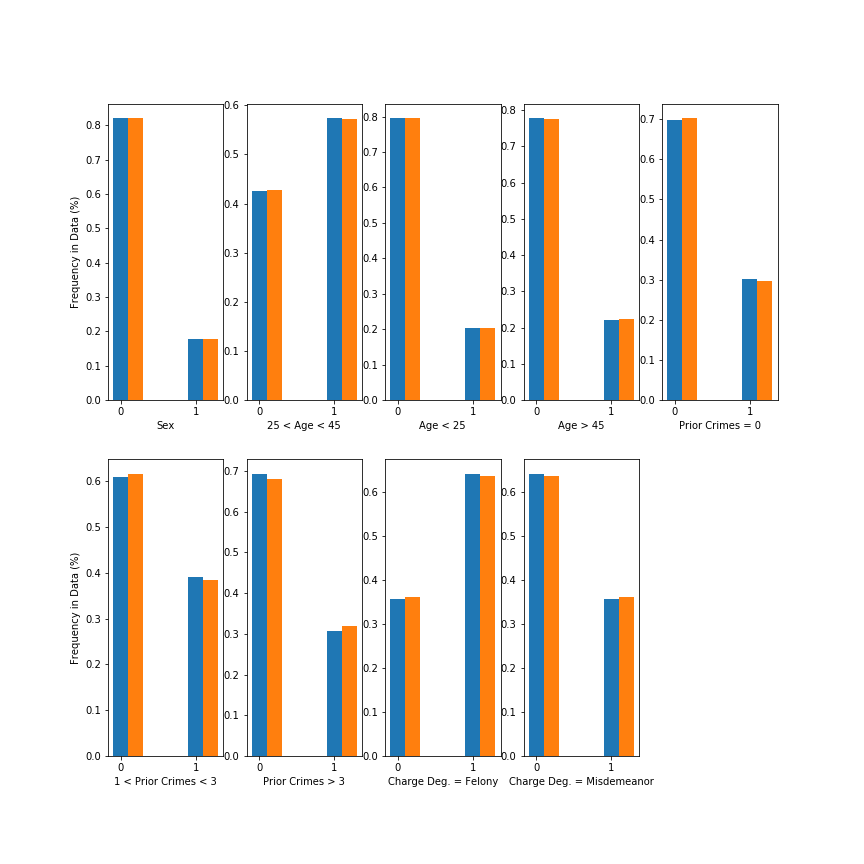
\includegraphics[scale=0.5]{marginals/compas_DP.png}
\captionof{figure}{COMPAS DP marginal distributions. Blue is unweighted ("fair"), orange is reweighted ("unfair"). \label{fig:img1}}
\vspace{5pt}
\par}

\subsection{COMPAS EO Marginal Distributions}

{\centering\vspace{10pt}
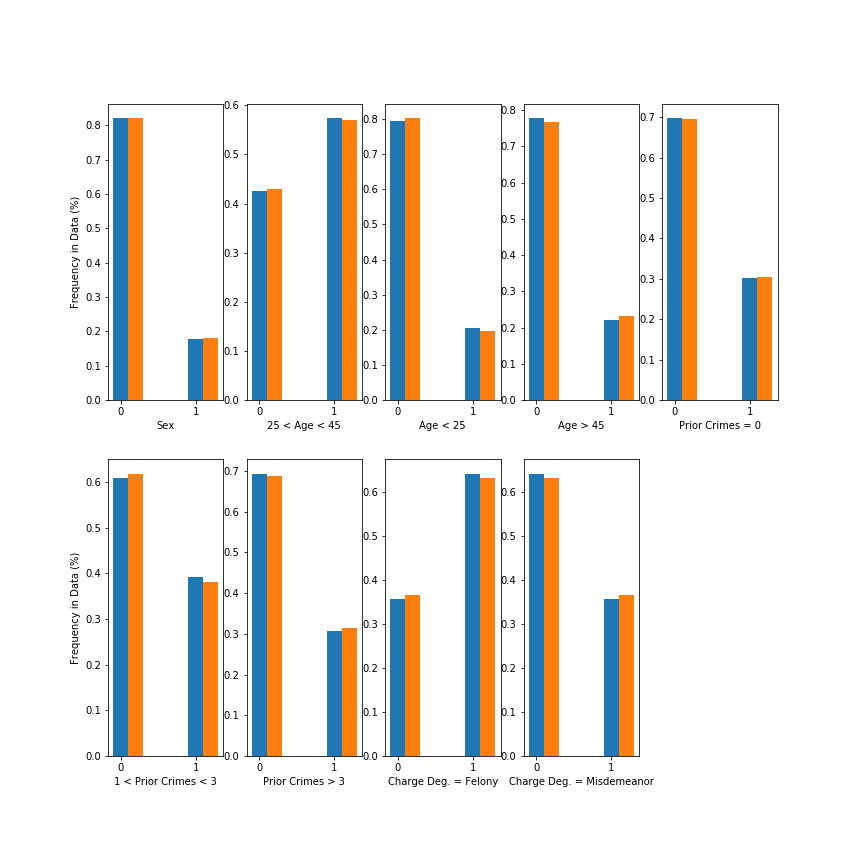
\includegraphics[scale=0.5]{marginals/compas_EO_Y0.png}
\captionof{figure}{COMPAS EO marginal distributions for $Y = 0$. Blue is unweighted ("fair"), orange is reweighted ("unfair"). \label{fig:img2}}
\vspace{5pt}
\par}

{\centering\vspace{10pt}
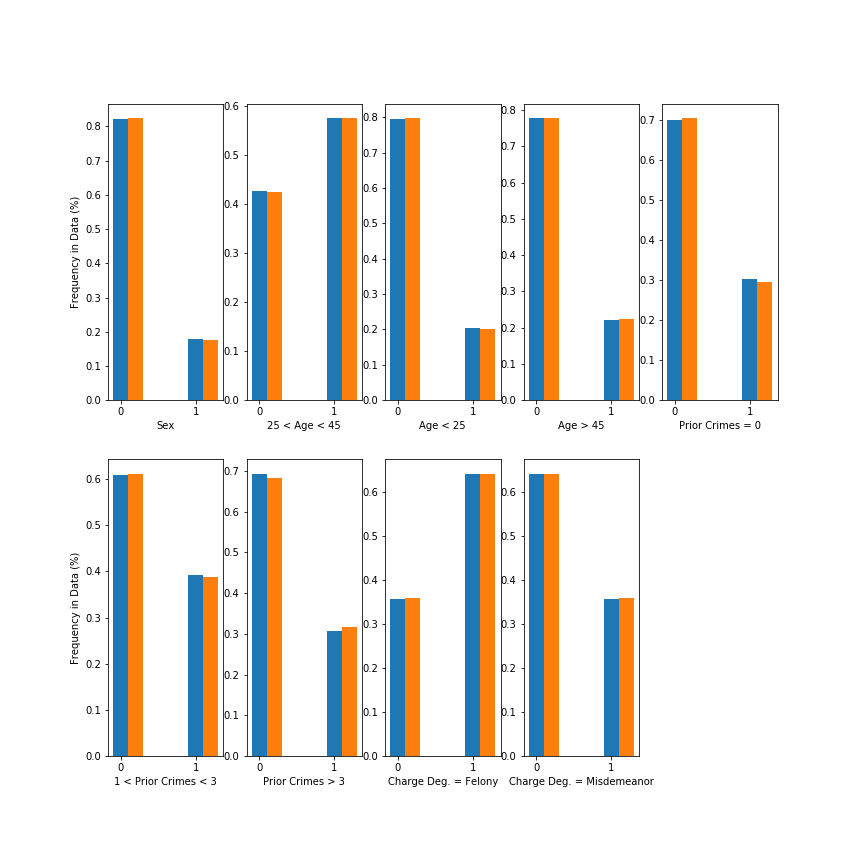
\includegraphics[scale=0.5]{marginals/compas_EO_Y1.png}
\captionof{figure}{COMPAS EO marginal distributions for $Y = 1$. Blue is unweighted ("fair"), orange is reweighted ("unfair"). \label{fig:img3}}
\vspace{5pt}
\par}

\subsection{Adult DP Marginal Distributions}

{\centering\vspace{10pt}
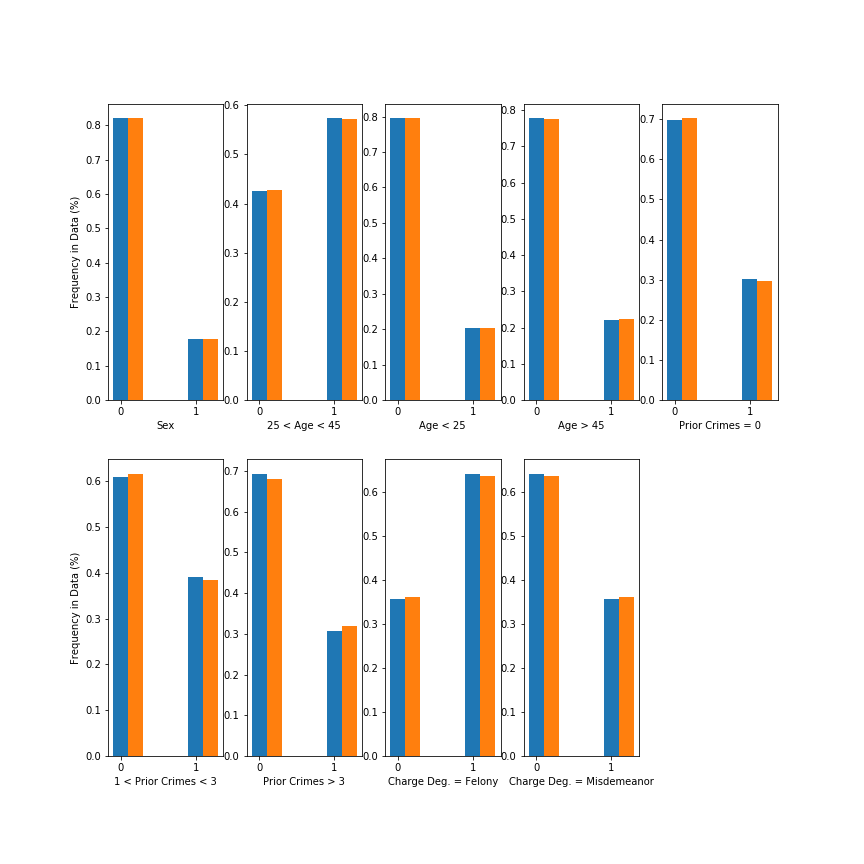
\includegraphics[scale=0.5]{marginals/compas_DP.png}
\captionof{figure}{Adult DP marginal distributions. Blue is unweighted ("fair"), orange is reweighted ("unfair"). \label{fig:img4}}
\vspace{5pt}
\par}

\subsection{Adult EO Marginal Distributions}

{\centering\vspace{10pt}
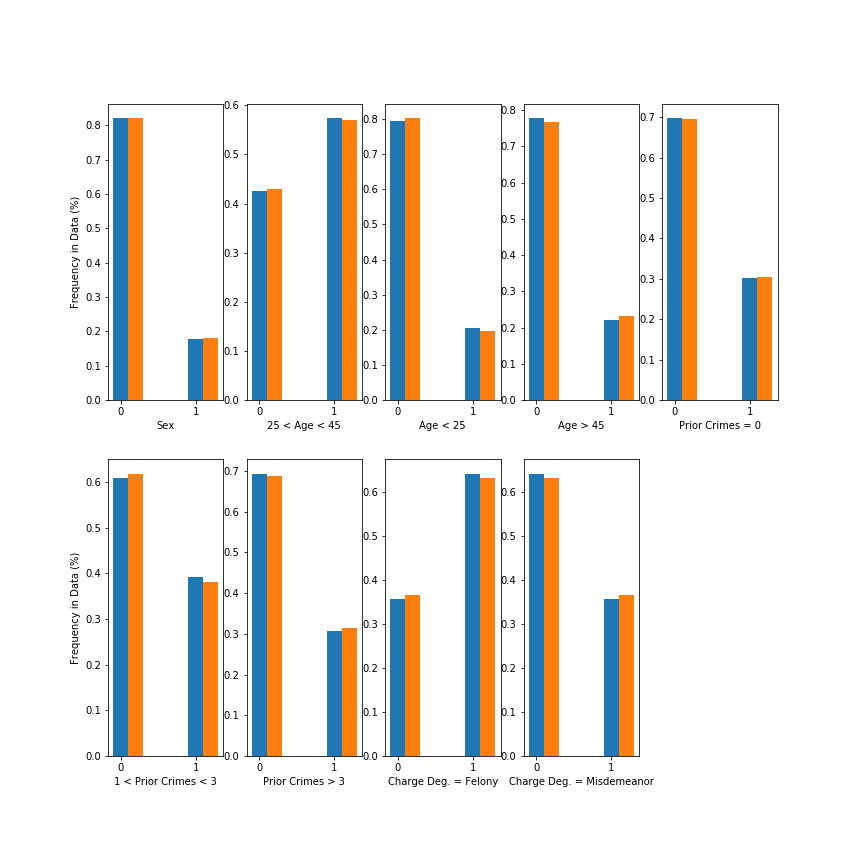
\includegraphics[scale=0.5]{marginals/compas_EO_Y0.png}
\captionof{figure}{Adult EO marginal distributions for $Y = 0$. Blue is unweighted ("fair"), orange is reweighted ("unfair"). \label{fig:img5}}
\vspace{5pt}
\par}

{\centering\vspace{10pt}
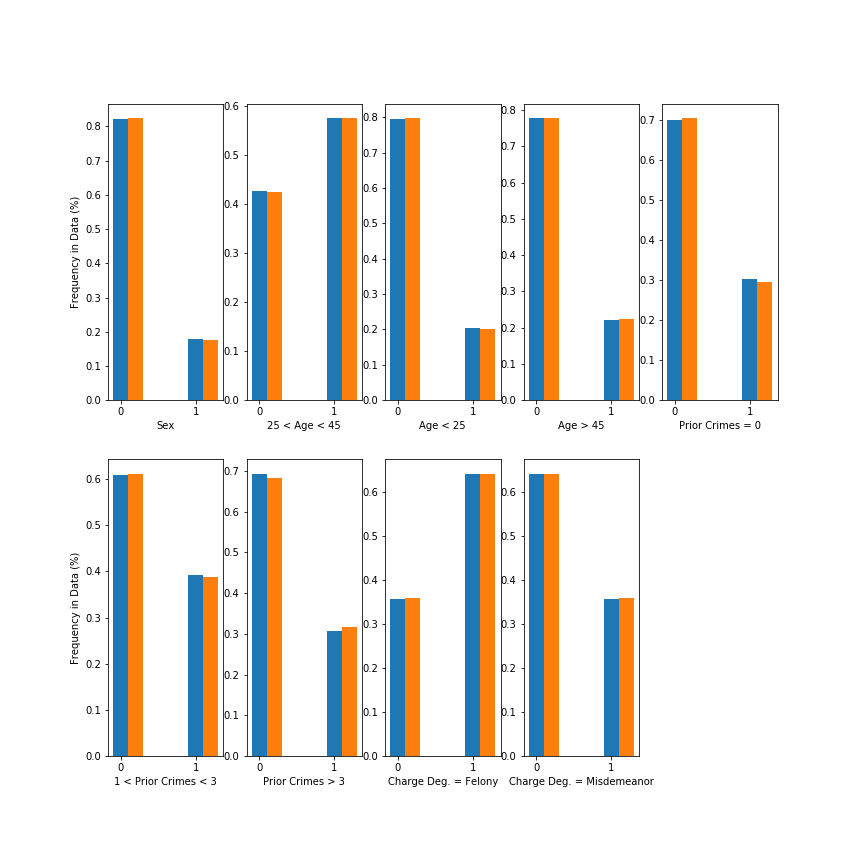
\includegraphics[scale=0.5]{marginals/compas_EO_Y1.png}
\captionof{figure}{Adult EO marginal distributions for $Y = 1$. Blue is unweighted ("fair"), orange is reweighted ("unfair"). \label{fig:img6}}
\vspace{5pt}
\par}
\end{document}